\documentclass[12pt]{article} % Corpo do texto em tamanho 12

% --- Configurações de Margem e Fonte ---
\usepackage[utf8]{inputenc}
\usepackage[T1]{fontenc}
\usepackage[a4paper, margin=2cm]{geometry} % Margem mínima de 2cm em todos os lados
\usepackage{times} % Fonte Times New Roman
\usepackage{xcolor}
\usepackage{listings}
\usepackage{graphicx}
\usepackage{fancyhdr}
\usepackage{hyperref}
\usepackage{titlesec} % Pacote para personalizar tamanhos de títulos
\usepackage{float}

% --- Configuração de Tamanho de Títulos ---
% Títulos de seção (14pt ou 16pt). Definido aqui como 16pt para destaque.
\titleformat{\section}{\normalfont\Large\bfseries}{\thesection}{1em}{}
\titleformat{\subsection}{\normalfont\large\bfseries}{\thesubsection}{1em}{}

% --- Configuração de Blocos de Código (Fonte Monoespaçada) ---
\definecolor{codebg}{gray}{0.95} % Fundo cinza claro
\lstset{
    basicstyle=\ttfamily\small, % Fonte monoespaçada
    backgroundcolor=\color{codebg},
    breaklines=true,
    frame=single,
    rulecolor=\color{black!30},
    showstringspaces=false,
    captionpos=b % Legenda abaixo do bloco
}

% --- Cabeçalho e Rodapé ---
\pagestyle{fancy}
\fancyhf{}
\fancyhead[L]{Bounty Hacker - Lurian Lima} % Nome do desafio e autor no cabeçalho
\fancyhead[R]{Write-Up}
\fancyfoot[C]{\thepage} % Numeração de páginas obrigatória

\begin{document}

% --- Capa ---
\begin{titlepage}
    \centering
    \vspace*{2cm}
    {\Huge \textbf{Write-Up de Segurança Ofensiva} \par}
    \vspace{1.5cm}
    {\Large \textbf{Desafio:} Bounty Hacker \par}
    {\large \textbf{Plataforma:} Try Hack Me \par}
    {\large \textbf{Autor:} Lurian Lima \par}
    \vspace{2cm}
    {\large \textbf{Data de Resolução:} \today \par}
    \vfill
\end{titlepage}

% --- Sumário ---
\tableofcontents
\newpage

% ---------------
% Resultados da enumeração. Use o comando abaixo para inserir screenshots:
% \begin{figure}[H]
%     \centering
%     \includegraphics[width=0.8\textwidth]{screenshot_nmap.png}
%     \caption{Legenda descritiva da imagem inserida imediatamente após o texto.}
% \end{figure}

% \begin{lstlisting}[caption={Comando de exploração utilizado}]
% # Exemplo de bloco de código com fundo destacado
% nmap -sV -sC -oN scan.txt 10.10.10.10
% \end{lstlisting}
% ---------------

% --- 2.3 Visão Geral ---
\section{Visão Geral}
% Parágrafo descrevendo o vetor principal de ataque sem spoiler detalhado. Deve responder: o que é o desafio,
% qual a superfície de ataque explorada e qual foi o caminho geral até o objetivo.

O desafio Bounty Hacker consiste em avaliar uma máquina Linux exposta na rede e identificar uma cadeia de exploração a partir dos serviços disponíveis. A enumeração inicial revelou serviços FTP, SSH e HTTP, com acesso anônimo habilitado no FTP. A partir dos arquivos disponibilizados nesse serviço, foi possível identificar informações que levaram ao acesso SSH como o usuário \textit{lin}. Após obter acesso ao sistema, a análise das permissões de sudo revelou que o binário \textit{tar} podia ser executado com privilégios de root, permitindo a escalada de privilégios e a obtenção da flag final.

% --- 2.4 Reconhecimento ---
\section{Reconhecimento}
% Resultados da enumeração externa: portas abertas, serviços identificados, versões relevantes, tecnologias
% detectadas. Incluir comandos usados e os trechos de output mais relevantes. Não incluir informações obtidas
% após o foothold inicial.

O primeiro passo é rodar o nmap:

\begin{lstlisting}[caption={Explorando o ip com nmap}]
nmap -sC -sV -T4 -p- <ip>
\end{lstlisting}

As opções utilizadas no comando significam:

\begin{itemize}
    \item \texttt{-sC}: executa os scripts padrão do Nmap para obter informações adicionais sobre os serviços.
    \item \texttt{-sV}: identifica as versões dos serviços encontrados nas portas abertas.
    \item \texttt{-T4}: utiliza um perfil de varredura mais rápido, adequado para redes estáveis.
\end{itemize}

\begin{lstlisting}[caption={Resultado do nmap}]
Not shown: 967 filtered tcp ports (no-response), 30 closed tcp ports (conn-refused)
PORT   STATE SERVICE VERSION
21/tcp open  ftp     vsftpd 3.0.5
| ftp-anon: Anonymous FTP login allowed (FTP code 230)
|_Can't get directory listing: PASV failed: 550 Permission denied.
| ftp-syst: 
|   STAT: 
| FTP server status:
|      Connected to ::ffff:192.168.129.184
|      Logged in as ftp
|      TYPE: ASCII
|      No session bandwidth limit
|      Session timeout in seconds is 300
|      Control connection is plain text
|      Data connections will be plain text
|      At session startup, client count was 2
|      vsFTPd 3.0.5 - secure, fast, stable
|_End of status
22/tcp open  ssh     OpenSSH 8.2p1 Ubuntu 4ubuntu0.13 (Ubuntu Linux; protocol 2.0)
| ssh-hostkey: 
|   3072 52:dd:4c:d0:15:5c:8d:04:2d:bd:2b:f5:a1:06:29:a4 (RSA)
|   256 1f:d6:99:6d:c0:b4:a7:d2:98:64:84:da:1b:99:4c:ad (ECDSA)
|_  256 89:a0:66:6d:79:f4:b2:d0:af:68:21:0a:69:65:92:34 (ED25519)
80/tcp open  http    Apache httpd 2.4.41 ((Ubuntu))
|_http-title: Site doesn't have a title (text/html).
|_http-server-header: Apache/2.4.41 (Ubuntu)
Service Info: OSs: Unix, Linux; CPE: cpe:/o:linux:linux_kernel
\end{lstlisting}

O resultado revela três serviços acessíveis: FTP na porta 21, SSH na porta 22 e HTTP na porta 80, todos executados em um sistema Linux. O serviço FTP utiliza o vsftpd 3.0.5 e permite login anônimo, o que representa o principal ponto de interesse da enumeração, embora a listagem de diretórios tenha sido bloqueada por uma falha na conexão passiva. Na porta 80, o Apache 2.4.41 responde, mas a ausência de um título indica que ainda é necessário realizar uma enumeração mais detalhada do conteúdo web. As portas restantes aparecem filtradas ou fechadas, reduzindo a superfície de ataque inicialmente disponível.

% --- 2.5 Exploração ---
\section{Exploração}
% Descrição técnica do vetor de entrada. Deve incluir o raciocínio que levou à identificação da vulnerabilidade,
% os payloads ou scripts utilizados (comentados), exploits públicos utilizados e os outputs que confirmam o
% acesso. Cada passo deve ser justificado, não apenas listado.

Após indentificarmos o servidor ftp, é possível acessá-lo via login anônimo.

\begin{figure}[H]
    \centering
    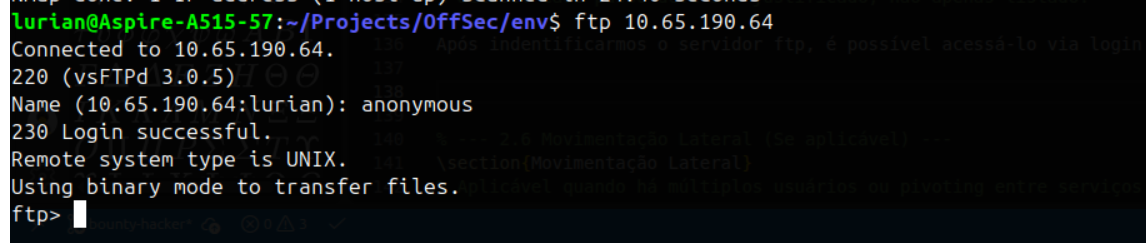
\includegraphics[width=0.8\textwidth]{imgs/ftp_login_anonymous.png}
    \caption{Logando no servidor ftp como anonymous.}
\end{figure}

Em seguida, podemos fazer um \textit{ls} para ver os arquivos existentes no server:

\begin{lstlisting}[caption={resultado da listagem de arquivos no servidor}]
ftp> ls
550 Permission denied.
200 PORT command successful. Consider using PASV.
150 Here comes the directory listing.
-rw-rw-r--    1 ftp      ftp           418 Jun 07  2020 locks.txt
-rw-rw-r--    1 ftp      ftp            68 Jun 07  2020 task.txt
226 Directory send OK.
\end{lstlisting}

Desse modo, podemos baixar os arquivos \textit{locks.txt} e \textit{task.txt}. Uma amostra do conteúdo de cada arquivo segue listado abaixo:

\begin{lstlisting}[caption={conteúdo do arquivo \textit{locks.txt}}]
rEddrAGON
ReDdr4g0nSynd!cat3
Dr@gOn$yn9icat3
R3DDr46ONSYndIC@Te
ReddRA60N
R3dDrag0nSynd1c4te
dRa6oN5YNDiCATE
...
\end{lstlisting}

\begin{lstlisting}[caption={conteúdo do arquivo \textit{task.txt}}]
1.) Protect Vicious.
2.) Plan for Red Eye pickup on the moon.

-lin
\end{lstlisting}

É bem provável que o arquivo \textit{locks.txt} seja uma lista de senhas de usuários. Portanto, o próximo passo é tentar logar como o \textit{lin} usando uma das senhas. 

Testando as senhas manualmente, é possível logar como \textit{lin} com a senha \textit{RedDr4gonSynd1cat3}

\begin{figure}[H]
    \centering
    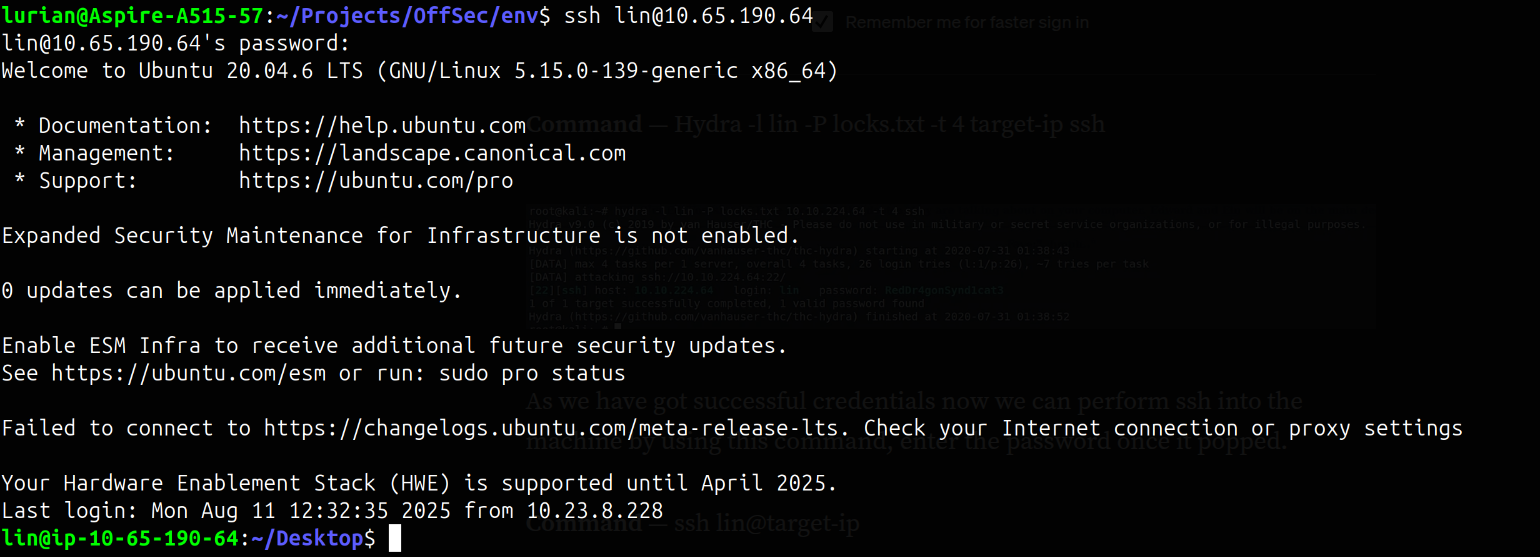
\includegraphics[width=0.8\textwidth]{imgs/login_lin_ssh.png}
    \caption{Logando como \textit{lin} no servidor ssh.}
\end{figure}

Ao fazer o login, é encontrado o arquivo user.txt, que contém a primeira flag.

% --- 2.7 Escalada de Privilégios ---
\section{Escalada de Privilégios}
% Descrever o vetor de privesc identificado, o processo de enumeração local que o revelou (linpeas, sudo -l,
% capabilities, etc.) e a exploração realizada. Incluir o comando final que comprova o acesso root/SYSTEM

É possível verificar os privilégios do usuário da seguinte forma:

\begin{figure}[H]
    \centering
    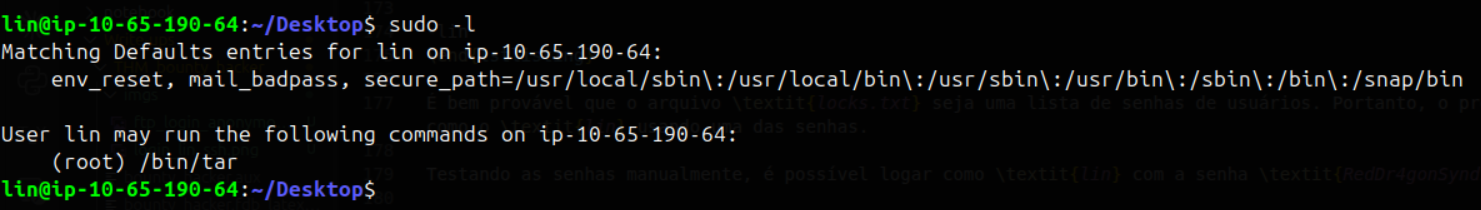
\includegraphics[width=0.8\textwidth]{imgs/sudo_l.png}
    \caption{Verificando os privilégios do usuário.}
\end{figure}

É possível ver que o usuário consegue executar \textit{/bin/tar} com os privilégios de root. No GTFOBins, podemos encontrar um comando com esse binário que escalar privilégios \footnote{https://gtfobins.org/gtfobins/tar/}.

\begin{figure}[H]
    \centering
    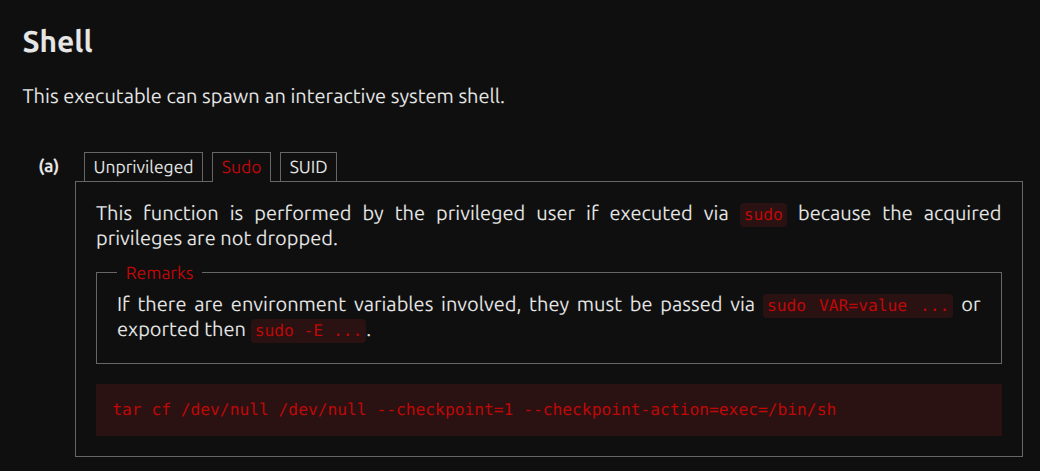
\includegraphics[width=0.8\textwidth]{imgs/scalete_privileges_gtfobins.png}
    \caption{Comando usando o binário tar para escalar privilégios.}
\end{figure}

Por fim, basta acessar a pasta root, onde estará a última flag.

% --- 2.8 Conclusão ---
\section{Conclusão}
% Resumo técnico de 3 a 5 linhas sintetizando a cadeia de exploração completa, do reconhecimento à flag.

A exploração começou com a enumeração das portas e serviços, que identificou o FTP com login anônimo habilitado. Os arquivos \textit{locks.txt} e \textit{task.txt} forneceram uma lista de senhas e a indicação do usuário \textit{lin}, possibilitando o acesso via SSH e a obtenção da flag de usuário. Em seguida, a consulta às permissões de sudo mostrou que o binário \textit{tar} podia ser executado como root. Utilizando essa configuração junto à técnica documentada no GTFOBins, foi possível elevar os privilégios e acessar a flag de root.

% --- 2.9 Referências ---
\section{Referências}
% Espaço destinado às fontes utilizadas para a exploração: links dos repositórios dos exploits públicos e links
% das CVEs correspondentes.

\begin{itemize}
    \item GTFOBins --- execução privilegiada do binário \textit{tar}: \url{https://gtfobins.org/gtfobins/tar/}
    \item Nmap Reference Guide --- documentação oficial do Nmap: \url{https://nmap.org/book/man.html}
    \item RFC 959 --- protocolo FTP (File Transfer Protocol): \url{https://www.rfc-editor.org/rfc/rfc959}
\end{itemize}

\end{document}